\chapter{Podaci}
\label{chap:podaci}

Orthobalancer radi sa primarnim proteinskim strukturama --- sekvencama
reziduuma, odnosno aminokiselina. Za zapis sekvenci koristi se standardizirani
FASTA format. Orthobalancer za svoj rad koristi dvije
NCBI-jevih\footnote{National Center for Biotechnology Information} baza
podataka od kojih jedna sadrži sekvence formatirane u FASTA format, a druga
taksonomsko stablo živog svijeta.


\section{FASTA format}
\label{sec:fasta}

FASTA je jedan od standardnih formata zapisa genetskih informacija na računalu.
Format je tekstualnog oblika, a koristi se u NCBI-jevim alatima i bazama
podataka, poput BLAST-a i neredundantne baze proteinskih sekvenci. Jedan zapis u
datoteci s FASTA sekvencama se sastoji od zaglavlja i sekvence. Zaglavlje je
jedan redak koji započinje s znakom '\texttt{>}' te nakon njega može imati razne
informacije koje opisuju dan zapis. Zapisi proteinskih sekvenci u NCBI-jevoj
neredundantnoj bazi obično imaju jedinstveni ključ sekvence, ime proteina, ime
vrste u kojoj se protein nalazi, podatke o originalnoj bazi i slično. Nakon
zaglavlja slijede retci koji sadrže zapisanu sekvencu gdje svaki znak
predstavlja jedan reziduum aminokiseline u peptidnom lancu. Kad bi ti se retci
slijepili zajedno, dobila bi se sekvenca u jednom nizu. Prazne linije nisu
dopuštene.


\section{Neredundantna baza}
\label{sec:nrdb}

Neredundantna baza je baza podataka koju nudi NCBI, a sadrži prikupljene zapise
iz nekoliko baza sa raznih instituta u svijetu, poput GenPept, Swissprot, PIR,
PDF, PDB i NCBI RefSeq. Za neredundantnu bazu se garantira da ne sadrži dvije
jednake sekvence, već se one tada spajaju u jedan FASTA zapis sa proširenim
zaglavljem.


\section{Taksonomsko stablo živog svijeta}
\label{sec:taxdb}

\emph{Taxonomy} baza, odnosno baza taksonomskog stabla živog svijeta
dostupna je u obliku nekoliko tekstualnih datoteka. Najbitnije, koje se koriste
u Orthobalanceru su \emph{nodes.dmp} i \emph{names.dmp}. Za svaki čvor stabla,
\emph{nodes.dmp} sadrži identifikacijski broj čvora, identifikacijski broj
roditelja te niz dodatnih informacija, poput ranga ovog čvora u stablu (carstvo,
rod, vrsta, \ldots). \emph{names.dmp} za svaki čvor čuva niz raznih imena, od
kojih je jedno jedinstveno, odnosno znanstveno, a ostala su prisutna za lakše
raspoznavanje od strane čovjeka.


\section{Ulaz}
\label{sec:input}

Aplikacija kao ulaz prima nekolicinu paralognih proteina u FASTA formatu. Ako
korisnik posjeduje samo sekvencu proteina, može ju zadati bez FASTA zaglavlja,
no u tome je slučaju dužan dati ime unesenoj sekvenci. Nužno je imati ime za svaki
ulazni paralog te je nužno da da su sva međusobno jedinstvena.

Dodatno, korisnik može specificirati čvorove taksonomskog stabla za čija
podstabla smatra da sadrže zamjenjive vrste. Ponuđen je i osnovni skup
zamjenskih čvorova za koje se vjeruje da bi mogli biti od koristi korisniku.


\section{Izlaz}
\label{sec:output}

Web aplikacija za završetak izvođenja prikazuje tablicu balansiranih vrsta.
Stupci tablice su imenovani po paralozima s ulaza. Retci su grupirani u
zamjenske čvorove. Svaki redak predstavlja jedan balansirani skup vrsta. U
stupcu pod pojedinim paralogom nalazi se ortologna vrsta, a lijevo od svih vrsta
je zapisan čvor na kojem su vrste tog retka balansirane. Primjer tablice se može
vidjeti naslici \ref{fig:tablica}.

\begin{figure}[h!]
\centering
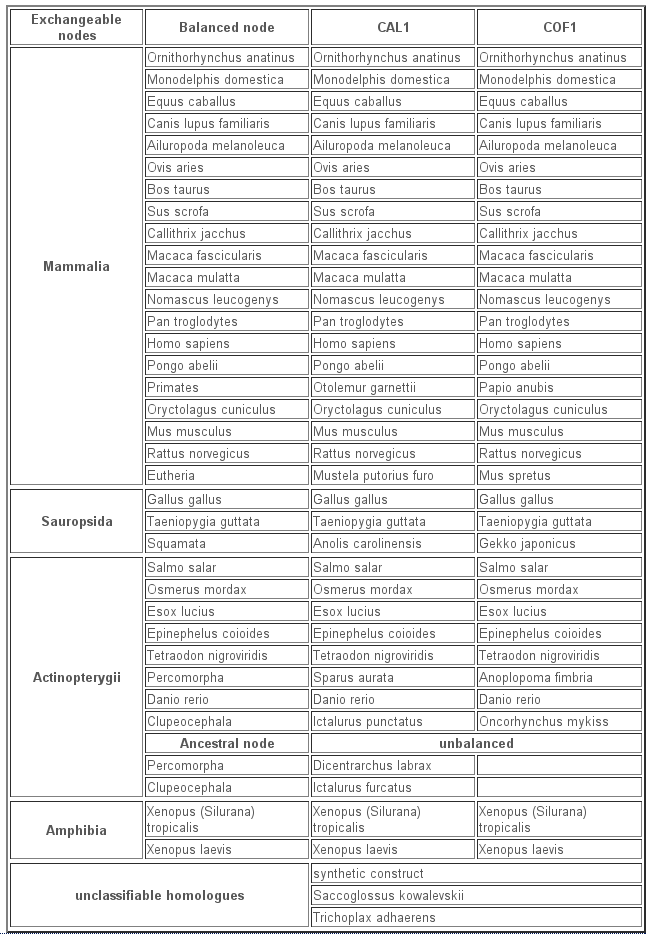
\includegraphics[width=4.75in]{figures/tablica.png}
\caption{Izlazna tablica sa web stranice Orthobanalcera}
\label{fig:tablica}
\end{figure}

Također, završna stranica sadrži poveznice za preuzimanje generiranih datoteka
tijekom izvođenja. Datoteke su opisane u nastavku.
